% This is samplepaper.tex, a sample chapter demonstrating the
% LLNCS macro package for Springer Computer Science proceedings;
% Version 2.20 of 2017/10/04
%
\documentclass{llncs}
%
\usepackage{graphicx}
% Used for displaying a sample figure. If possible, figure files should
% be included in EPS format.
%
% If you use the hyperref package, please uncomment the following line
% to display URLs in blue roman font according to Springer's eBook style:
% \renewcommand\UrlFont{\color{blue}\rmfamily}

\usepackage{hyperref} % for url
\usepackage{pythonhighlight} % for python

%% listings for python
\usepackage{xcolor}     %高亮使用的颜色
\definecolor{commentcolor}{RGB}{85,139,78}
\definecolor{stringcolor}{RGB}{206,145,108}
\definecolor{keywordcolor}{RGB}{34,34,250}
\definecolor{backcolor}{RGB}{220,220,220}
\usepackage{accsupp}    
\newcommand{\emptyaccsupp}[1]{\BeginAccSupp{ActualText={}}#1\EndAccSupp{}}
\usepackage{listings}
\lstset{                        %高亮代码设置
    language=python,                    %Python语法高亮
    linewidth=0.9\linewidth,            %列表list宽度
    %basicstyle=\ttfamily,              %tt无法显示空格
    commentstyle=\color{commentcolor},  %注释颜色
    keywordstyle=\color{keywordcolor},  %关键词颜色
    stringstyle=\color{stringcolor},    %字符串颜色
    %showspaces=true,                   %显示空格
    numbers=left,                       %行数显示在左侧
    numberstyle=\tiny\emptyaccsupp,     %行数数字格式
    numbersep=5pt,                      %数字间隔
    frame=single,                       %加框
    framerule=0pt,                      %不划线
    escapeinside=@@,                    %逃逸标志
    emptylines=1,                       %
    xleftmargin=3em,                    %list左边距
    backgroundcolor=\color{backcolor},  %列表背景色
    tabsize=4,                          %制表符长度为4个字符
    gobble=4                            %忽略每行代码前4个字符
    }

\begin{document}
%
\title{A Short Instruction for \sf{nnbarrier}}
%
%\titlerunning{Abbreviated paper title}
% If the paper title is too long for the running head, you can set
% an abbreviated paper title here
%
\author{Hengjun Zhao}

\institute{School of Computer and Information Science\\
Southwest University, Chongqing, 400715, P.~R.~China\\
\email{zhaohj2016@swu.edu.cn}}
%
\maketitle % typeset the header of the contribution
%
% \begin{abstract}
% To be completed
% %\keywords{First keyword  \and Second keyword \and Another keyword.}
% \end{abstract}
%
%
\section{Introduction}
In our paper \emph{Synthesizing Barrier Certificates Using Neural Networks} accepted by HSCC'20, we developed a tool named \textsf{nnbarrier}
that can automatically learn a barrier ceritificate represented by a neural network for the safety verification of a continuous dynamical system. 
Here we give a short instruction to the use of \textsf{nnbarrier}, covering the system requirements, installation process, the structure of source codes,
sample inputs, and user-defined inputs. We will emphasize what parts that were presented in the submitted paper will be covered in the instruction, for the purpose of repeatability
evaluation. If there is any problem in using \textsf{nnbarrier}, please contact \email{zhaohj2016@swu.edu.cn}.

\section{Installation}
\begin{itemize}
\item What elements of the paper are included in the REP (e.g.: specific figures, tables, etc.).
\item The system requirements for running the REP (e.g.: OS, compilers, environments, etc.).
\item Instructions for installing and running the software and extracting the corresponding results. 
\end{itemize}

\begin{itemize}
    \item hscc2020 hscc20:111111
    \item ubuntu: 18.04.02 LTS \url{https://ubuntu.com/download/desktop}
    \item gcc: sudo apt update; sudo apt install build-essential; gcc --version
    \item python: 3.6.7 python3 --version \pyth{__init__}
    \item pip3: sudo apt install python3-pip
    \item git: sudo apt install git
    \item pytorch 1.3.1 cpu, torchvision 0.4.2 cpu: \url{https://pytorch.org/} \begin{verbatim}pip3 install torch==1.3.1+cpu torchvision==0.4.2+cpu -f 
    https://download.pytorch.org/whl/torch_stable.html\end{verbatim}
    \item python package: numpy, matplotlib \url{https://matplotlib.org/} \url{https://matplotlib.org/users/installing.html}
    \item mayavi \url{http://docs.enthought.com/mayavi/mayavi/} \url{http://docs.enthought.com/mayavi/mayavi/installation.html#installing-with-pip}
\end{itemize}

\begin{python}
    if i==0:
        abc
    else:
        def
\end{python}

\section{Sample Input}

\inputpython{../ann.py}{2}{5}

\section{Cases in the Paper}

\section{Define Your Own Problem}

\section{Fine-Tuning}

\subsection{A Subsection Sample}

Please \cite{Prajna04safetyverification} try \cite{BarryICRA2012} avoid rasterized images for line-art diagrams and
schemas. Whenever possible, use vector graphics instead (see
Fig.~\ref{fig1}).

\begin{figure}
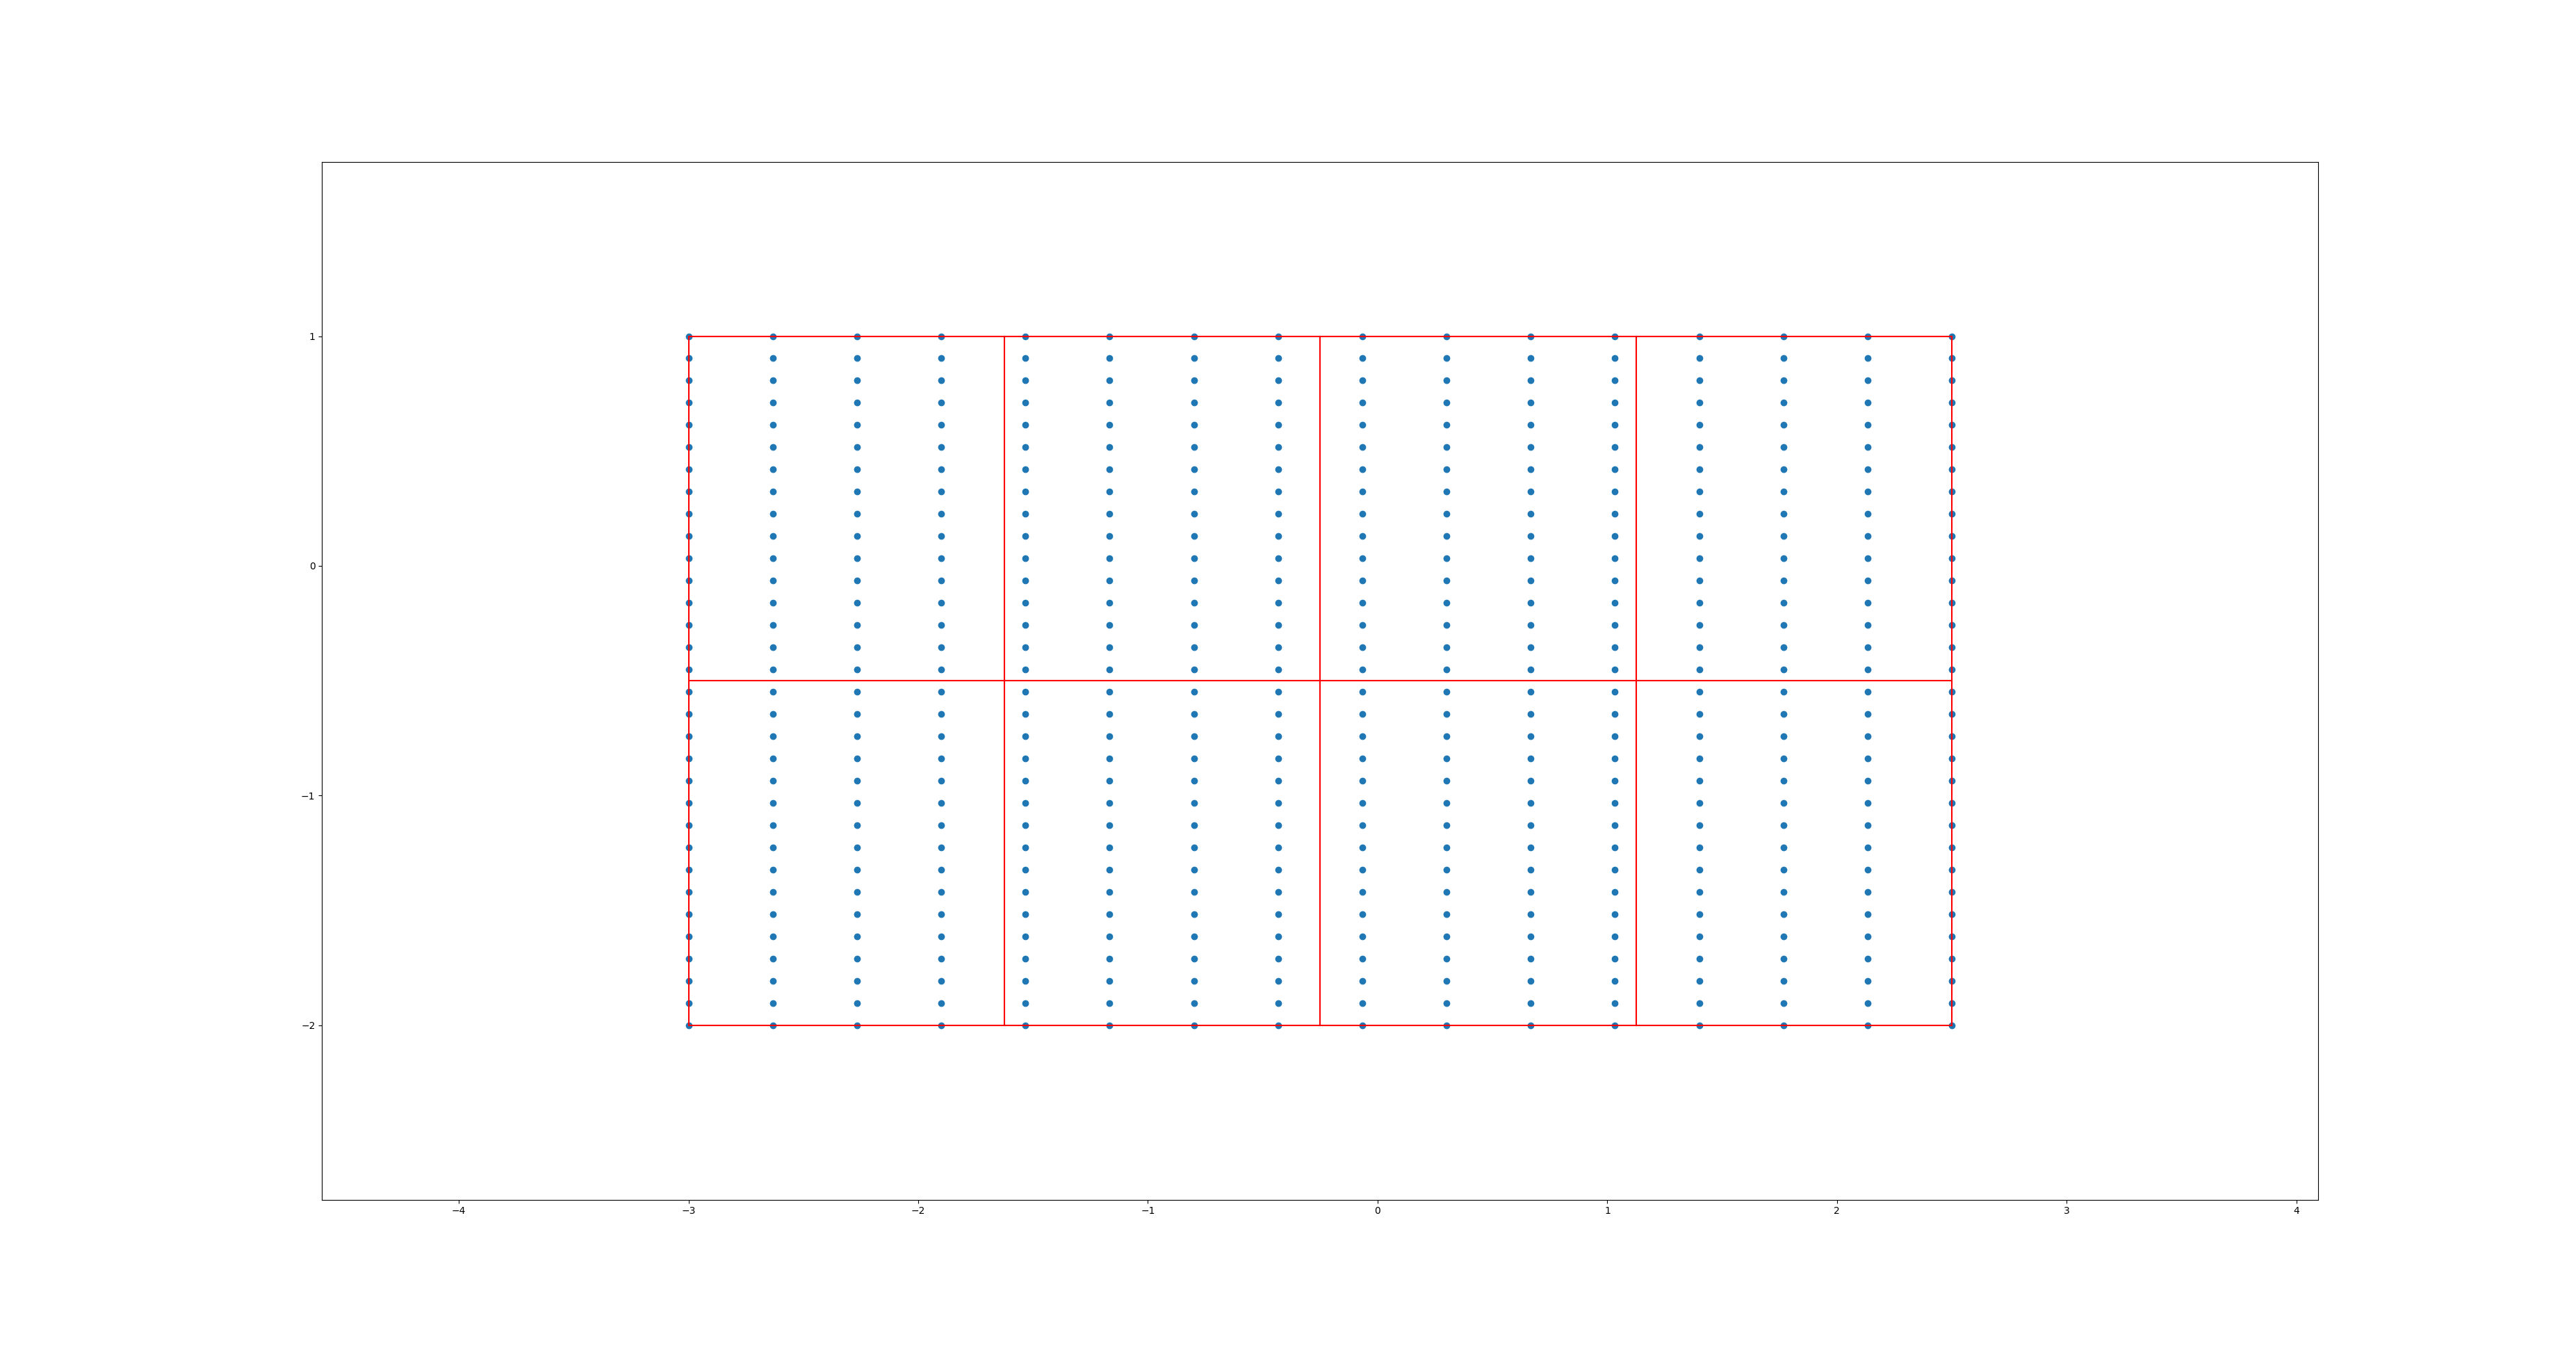
\includegraphics[width=\textwidth]{./fig/batch_data}
\caption{A figure caption is always placed below the illustration.
Please note that short captions are centered, while long ones are
justified by the macro package automatically.} \label{fig1}
\end{figure}

\bibliographystyle{splncs04}
\bibliography{instruction}

% \begin{thebibliography}{8}
% \bibitem{ref_article1}
% Author, F.: Article title. Journal \textbf{2}(5), 99--110 (2016)
% \end{thebibliography}

\end{document}
